

\chapter{Materials and Methods}
\label{chap:materials_methods}

\section{Working Environment and Technologies}
\label{sec:working_environment_and_technologies}
The work performed in this thesis was developed at the Department of Biology\footnote{\href{http://dept.bio.unipd.it/}{http://dept.bio.unipd.it/}} of the University of Padua\footnote{\href{http://www.unipd.it/}{http://www.unipd.it/}}. The available hardware used to test the performance of the implemented method is a cluster of eight computers. Each of them is characterized by a bi-processor Intel Xeon 2.80GHz CPU with 2GB RAM. The objective of the installed cluster is to perform grid computing. Grids serve to manage the allocation of jobs to computers which will perform the work independently of the rest of the cluster. While each job is not affected by other jobs in progress on other nodes of the grid, in this installation, resources are shared by all nodes. In addition to these machines, a laptop computer is used as terminal to access remotely each cluster node. The latter is an AMD Turion64 X2, 1.60GHz CPU with RAM 2GB. Figure \ref{fig:cribi} illustrates the work architecture.\\
The method implemented during this thesis is experimental because, despite the clearly defined goal, the way to achieve a good solution depends highly on results. Due to this difficulty, a more agile approach with the aim to encourage frequent inspection and adaptation is used instead of standard project planning. Agile methodologies choose to do things in small increments with minimal planning, rather than long-term planning. Iterations are short time frames which typically last from one to four weeks. Each iteration is led by a team through a full software development cycle, including planning, requirements analysis, design, coding, unit testing, and acceptance testing when a working product is demonstrated to stakeholders. This helps to minimize the overall risk, and allows the project to adapt to changes more quickly. A SCRUM-based approach is adopted to manage and solve this problem. A high-level document for the entire project, called in the SCRUM terminology \emph{product backlog}, is defined at the beginning of the thesis and continuously monitored, in order to satisfy the main objectives and control eventual drifts. It contains a list of backlog items that are broad descriptions of all required features and wishlist items. The \emph{product backlog} answers to \emph{what} will be done. It also presents rough estimates of both business value and development effort that help to gauge the timeline and to manage priorities. Then, a more detailed short job document, called \emph{sprint backlog}, is written with the aim to describe detailed information about \emph{how} to implement the requirements for the upcoming sprint. In this thesis, each job is broken down into quarters (a quarter corresponds to two hours of work). For each job, estimated and measured times must be provided. Also, jobs can be made by human, e.g. programming or testing a software module, or by machine, e.g. computing an optimization. Finally, a priority is associated to each job with the aim to schedule an order among the activities. \\
The generation of different datasets and automatic execution over a set of targets is implemented in the Perl v5.8 programming language. Much of the source code requires the manipulation of strings and pattern matching functionalities. Moreover, an important non-functional requirement is also that a molecular biologist must be able to alter the source code in the near future. Perl is a high-level, interpreted scripting language that provides powerful facilities for text processing and manipulation of text files. It is a programming language also known by biologists, allowing to execute and manipulate variants of this current implementation in the future. Rather, all modules regarding the effective computation, such as neural networks and clustering, are implemented in C++ programming language for performance reasons. \\
From a software point of view, the Debian GNU/Linux distribution is used with the installed compiler GCC v4.1. The method realized during this thesis will become a package, called Osiris, of the \gls{VICTOR} library. It also depends on the \gls{FANN} v2.0 that offers lots of functions to deal with training and test sets of neural networks in an easy and versatile way, leaving to the user the configuration and validation tasks. In order to program all source code, the GNU Emacs v2.22.1 editor is chosen due to its usability and configurability. Statistics plots and tables shown in this thesis are generated using the GNU R package\footnote{Source: \href{http://www.r-project.org/}{http://www.r-project.org/}}, a free software environment for statistical computing and graphics, and the software Gretl v1.7.5\footnote{Source: \href{http://gretl.sourceforge.net/index.html}{http://gretl.sourceforge.net/index.html}}. UML diagrams are generated using Eclipse v3.4.2 IDE.
\begin{figure}[tb]
	\begin{center}
		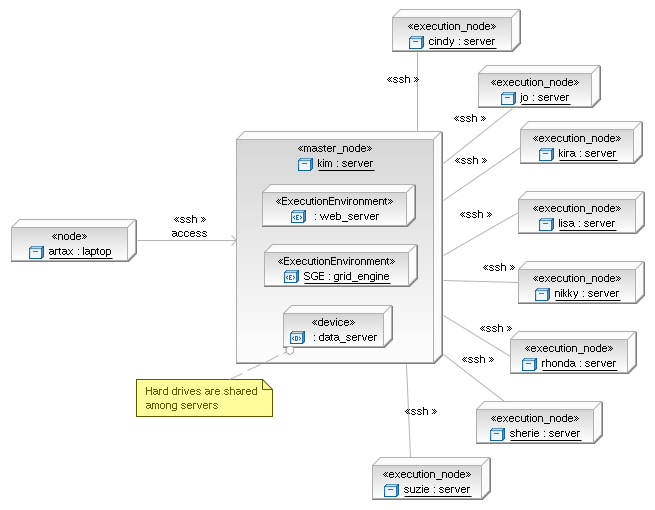
\includegraphics[scale=0.85]{cribi}
		\caption[Cluster of computers at CRIBI]{UML deployment diagram. All data resources are shared and located inside the Kim server. Every executive node is visible and accessible only by the Kim server which represents the master node. Registered users can run processes by SSH connection, all others by web interface if the web service is available.}
		\label{fig:cribi}
	\end{center}
\end{figure}



\section{How to Improve QMEAN}
\label{sec:howto_improve_qmean}
QMEAN \cite{Benkert2007, Benkert2008ab, Benkert2008aa, Tosatto2002} is a single-model scoring function based on a linear combination of a set of statistical potentials. A brief presentation dealing with statistical potentials is provided in Appendix \ref{sec:statistical_potentials}. The original idea of using such a scoring function composed by statistical potentials is found in \glslink{FRST}{FRST} \cite{Tosatto2005}. The last version of QMEAN scoring function, that is QMEAN6, can be described as follows:
\begin{equation}
	score = f(P_1, P_2, \ldots, P_6) = P_1w_1 + P_2w_2 + \ldots + P_6w_6
\end{equation}
where the vector \(\vec{P} = (P_1,P_2,\ldots,P_6)\) contains six features computed by QMEAN and the weight vector \(\vec{W} = (w_1,w_2,\ldots,w_6)\) is performed on the CASP-6 training set by using linear regression as implemented in the R package with the GDT\_TS score as target function.\\
The six features computed by QMEAN are the following:
\begin{description}
\item[Torsion 3-residue.] Extended torsion potential based on $\phi$ and $\psi$ propensities over three consecutive residues. Bin sizes: 45\textdegree\space for the center residue, 90\textdegree\space for the two adjacent residues.
\item[Solvation $C_\beta$.] Potential reflecting the propensity of a certain amino acid for a certain degree of solvent exposure based on the number of $C_\beta$ atoms within a sphere of 9 \AA{} around the center $C_\beta$.
\item[Pairwise $C_\beta$/SSE.] Residue specific pairwise distance dependent potential using $C_\beta$ atoms as interaction centers. Range 3-25 \AA{}, step size: 0.5 \AA{}. A secondary structure specific implementation was used both for the derivation and application of the potential.
\item[All-atom distance-dependent interaction.] Secondary structure specific interaction potential using all 167 atom types. The range is 3-20 \AA{} and the step size is 0.5 \AA{}.
\item[SSE PSIPRED.] Agreement between the predicted secondary structure of the target sequence using PSIPRED \cite{Jones1999aa} and the observed secondary structure of the model as calculated by the program \gls{DSSP} \cite{Kabsch1983aa}.
\item[ACCpro.] Agreement between the predicted relative solvent accessibility using SSPROACC \cite{Pollastri2007aa, Schuster1997aa} and the relative solvent accessibility derived from DSSP.
\end{description}
On the other hand, the weight vector is used to weight each parameter computed from the current protein model. The optimized weight vector is defined as:
\begin{equation}
\vec{W} = 
\left(
\begin{array}{c}
	w_{Torsion}\\
	w_{Solvation}\\
	w_{Pairwise}\\
	w_{All-atom}\\
	w_{SSE agreement}\\
	w_{ACC agreement}
\end{array}
\right) 
=
\left(
\begin{array}{c}
	-0.00185\\
	-0.00054\\
	-0.00062\\
	 -0.00108\\
	0.38072\\
	0.57997
\end{array}
\right)
\end{equation}

A scoring function of this type is immediate to implement and provides good solutions, even though it could be improved. Four possible ways to achieve this objective are described as follows:

\begin{description}
 \item[Non-Linear Method.] Different tertiary structure predictors are used to generate models for a given target sequence. Values computed from statistical potentials, which describe model properties, do not necessarily assume a linear behavior because they are depending on the model. For this reason, a non linear method should outperform the current linear weighed combination approach. In order to learn weights with the aim to deal with non-linear data, a \gls{SVM} or an \gls{ANN} could be used to.
 \item[Target Categorization.] QMEAN assumes input data quality to be uniformly distributed, while it is known that low quality models are much more fragment than median and high quality ones. A solution to this problem would be to consider different protein target classes separately. 
 \item[Using Density Information.] QMEAN is a single-model method, so it does not take into account density information. QMEANclust, the clustering version of QMEAN, was implemented because clustering-based methods perform better, as previously shown in \S~\ref{subsec:clustering_based_methods}. Therefore, it would be relevant and interesting to study a new strategy to include density information in the score computation.
 \item[Addition of New Features.] A good set of features describing the protein model forms the basis for a good single-model method. It is important that chosen features to be orthogonal among each other because the aim is to summarize well all main aspects of the predicted model. The research of new useful parameters could outperform the actual method.
 \end{description} 

\section{Description of the Osiris Package}
\label{sec:a_raw_neural_network}
The implemented system takes into account all previously cited improvements because:
\begin{itemize}
\item substitutes the QMEAN scoring function by using ANNs;
\item defines the quality of a model by considering its class also;
\item uses density information from an ensemble of models;
\item adopts other features in addition to those computed by QMEAN.
\end{itemize}
The study of ANNs has been inspired from information processing inside biological neural systems. In a neural network model, simple nodes, also called neurons or units, are connected together to form a network. ANNs are employed in statistics, cognitive psychology and artificial intelligence.\\
In this work, ANNs are trained following the supervised learning paradigm. In supervised learning, the network is trained by providing it with input and matching output patterns. These input-output pairs, also called training examples, are usually provided by hand or generated by a system component (self-learning). After this phase, network weights, inspired by neural synapses, are fixed and the system is ready to predict outputs from input samples. Most of the algorithms used in training artificial neural networks employ some form of gradient descent. A commonly used cost function is the \gls{MSE} which tries to minimize the average squared error between the network's output, $f(x)$, and the target value $y$ over all the example pairs. The most famous training algorithm based on gradient descent is backpropagation.\\
In order to capture density information on a data ensemble, clustering techniques are often used. Clustering is based on an unsupervised learning paradigm. In unsupervised learning, outputs are achieved by considering the relationships among a set of samples. Traditionally, clustering is referred to the assignment of objects into groups, called clusters, by computing a similarity or distance measure among objects.\\
More details on ANNs and clustering techniques are discussed in \cite{Baldi2001aa}, \cite{Mitchell1997aa}. The following subsections describe the system.

\subsection{Dataset Preprocessing}
\label{subsec:dataset_preprocessing}
The problem that MQAPs attemp to solve is quite particular. In fact, it requires the predictor to be quite general, but also able to distinguish little differences among models. To overcome these difficulties, a wide dataset is built in order to learn networks with a satisfactory number of samples.\\
In basic mode, features are represented by six parameters computed by QMEAN as shown in Figure \ref{fig:raw_ann}. They contain orthogonal information, meaning that each of them is independent enough from the others, and are not redundant. In all MQAPs, the output is a single real value in $[0, 1]$. Therefore, each ANN presents only an output unit, while the number of input units depends on how many features are considered. In order to build the dataset for the ANN, some previous activities are required. As shown in Figure \ref{fig:qmean_feature_generation}, it first needs to retrieve a target sequence $s$, a set of target models $M$ and the native structure $n$ related to the target sequence. QMEAN mainly requests three input parameters to execute:
\begin{description}
 \item [A target path:] a path containing a set of models $M$, in \gls{PDB} format, generated by tertiary structure predictors using the sequence $s$.
 \item [A file (*.horiz):] a file containing the secondary structure prediction of $s$, obtained by executing the program PSIPRED \cite{Jones1999aa}.
 \item [A file (*.sspro\_acc):] a file containing the secondary structure and solvent accessibility predictions of $s$, obtained by executing the program SSPROACC \cite{Pollastri2007aa, Schuster1997aa}.
\end{description}
The native structure and the TMscore program \cite{Zhang2004} are required in order to obtain the true model score, which serves in the learning phase.
\begin{figure}[tb]
	\begin{center}
		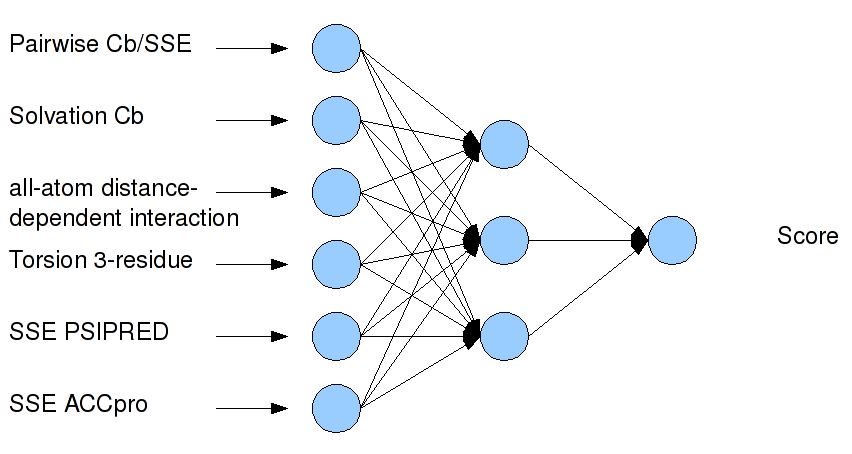
\includegraphics[scale=0.50]{raw_ann}
		\caption[Artificial neural network of six features from QMEAN]{Example of a simple ANN that receives as input six QMEAN features characterizing a model and returns a single output value that is the respective score.}
		\label{fig:raw_ann}
	\end{center}
\end{figure}
\begin{figure}[tb]
	\begin{center}
		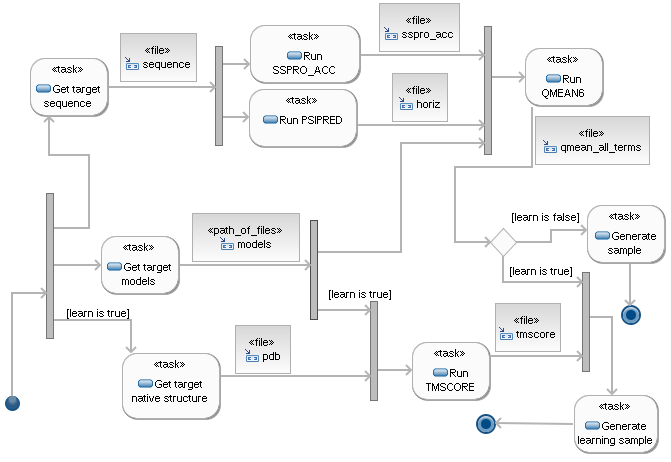
\includegraphics[scale=0.80]{qmean_feature_generation}
		\caption[Dataset generation UML diagram]{Conceptual activity UML diagram describing the key steps in order to obtain the dataset for the ANN. The procedure illustrated is summarised for one target and shows the data flow from the downloading step to the ANN dataset generation. Two areas could be distinguished: the QMEAN execution with the relative dependences and the TMscore execution. The first one is needed in order to obtain the six QMEAN features, while the second one is required when examples are used for learning the ANN, since it allows to associate the real model score. Therefore, in an operative phase of the ANN, the part of this diagram representing the TMscore execution is ignored. QMEAN features are scaled before being applied.}	
		\label{fig:qmean_feature_generation}
	\end{center}
\end{figure}

All target models used for training, that completely match another model of the same target are removed. In fact, it may happen that, for some different target models, QMEAN returns the same tuple of statistical potentials. For this reason, it is better to remove these redundant samples because they would deceive learning about the true data density distribution.\\
Since each QMEAN feature $f \in F$, where $F$ is the feature space, is defined in its own specific range, the values associated to that feature $f$ are previously scaled into the interval $[0, 1]$, before being used, in the following way:
\begin{enumerate}
 \item For each model $m \in M$, where $M$ is the set of all models of all target sequences, extract the previously computed value $v_f^{(m)}$ of the QMEAN feature $f$ and put it into vector $\vec{E}_f$.
 \item Store the minimum and the maximum value of the vector $\vec{E}_f$ in the variables $min_f$ and $max_f$ respectively.
 \item Compute the vector $\vec{N}_f$ by normalizing the vector $E_f$:
       \begin{equation}
       \label{eq:feature_normalization}
 	 \vec{N}_f(i) = \frac{\vec{E}_f(i) - min_f}{max_f - min_f}
       \end{equation}
       where $\vec{E}_f(i)$ is the $i$-th value of the vector $\vec{E}_f$, or in other words the value $v_f^{(m_i)}$ of the QMEAN feature $f$ computed for the $i$-th target model. 
\end{enumerate}
It is important to highlight that the minimum and maximum values of the feature $f$, respectively $min_f$ and $max_f$, are computed from data used for training, and stored in a file, with the aim to scale test data at a later time. Given a model used for testing the network, if the value associated to a feature $g$, overflows or underflows the admissible maximum or the minimum values for that feature, then that value will be approximated to $max_g$ in the overflow case or to $min_g$ otherwise.\\

\subsection{Training, Validating and Testing Phases}
\label{subsec:training_and_testing_phases}
During the learning phase, it is common to deal with two aspects: ANN selection and performance estimation. The former represents the choice of the \emph{optimal} parameters, e.g. learning parameters, network size and weights, for a certain classification or regression problem. The latter describes how to estimate the performance of the selected ANN.\\
The dataset is split into three subsets: 
\begin{itemize}
 \item Training set (TR): a set of examples used for learning over a certain tuple of classifier parameters.
 \item Validation set (VA): a set of examples used to tune the best tuple of classifier parameters.
 \item Test set (TE): a set of examples used only to assess the performance of a fully-trained classifier.
\end{itemize}
In order to train, validate and test the network, two different strategies can be considered: by target or by model. The first consists of considering each ANN sample as a target (which is composed of models), while the second one handles each sample as a model. The first strategy is chosen because allows a more effective distinction in samples used for training, validation or testing. In fact, it is possible that a subset of models generated for a certain target $t$ to be very similar. By considering ANN samples as protein models, the risk is to scatter two or more similar target models into two different subset, e.g. TR and VA, with the serious possibility of overestimating the network performance.\\
The training and validation sets are obtained by data from CASP-5, CASP-6 and CASP-7 (214 targets for a total of 78,854 models), while the test set is taken from CASP-4 (40 targets comprising 4,221 models) and CASP-8 (117 targets comprising 29,064 models). The test and validation sets are separated because it is known that the error rate estimate of the final model on validation data will be biased (lower than the true error rate) since the validation set is used to select the final ANN. The main procedure used to train, validate and test the network implemented is the following:
\begin{enumerate}
 \item Divide all the data into three partitions: training, validation and test set.
 \item Select the architecture and training parameters.
 \item Train the ANN using the training set.
 \item Evaluate the ANN using the validation set.
 \item Repeat step 2 through 4 using different architectures and training parameters.
 \item Select the best ANN and train it using data from the training and validation set.
 \item Assess this final ANN using the test set.
\end{enumerate}
Since K-fold cross validation is applied, steps 3 and 4 are repeated for each of the K folds. Then, the best ANN, see the $6^{th}$ step above, is the network having the minimum MSE (the minimum over a set of averaged MSEs obtained in step 4). The following subsections describe in detail the components of the procedure described above.

\subsubsection{Training}
\label{subsubsec:training}
All adopted ANNs are feed-forward. In feed-forward neural networks, the information moves in only one direction (forward) from the input, through the hidden to the output nodes without recurring cycles. The training algorithm used is Resilient backpropagation, Rprop, a local adaptive learning algorithm. Rprop is choosen with respect to other training algorithms such as Batch, Incremental or Quickprop for a series of reasons. First, it reduces the number of freely adjustable parameters, e.g. the learning rate, a problem that leads to a tedious search in the parameter space. Second, it is commonly considered a fast general purpose training algorithm. Third, it gives the best performance in the current described method. More details about the Rprop algorithm can be found in \cite{Riedmiller1994, Riedmiller1992}. Initial weights are small random values comprised in the real range $[-0.1, 0.1]$ in order to improve the gradient descent from a numerical point of view. The training stop function used is the MSE, set to suspend training when the desired error is 0 unless the maximum or stagnation number of epochs are reached. 
Two training modes are investigated: 
\begin{itemize}
 \item Fixed topology training. The training phase aims to find the \emph{optimal} weights by using a backpropagation-based training algorithm. All fixed topology ANNs trained in this work are composed by only one hidden layer, obtaining in this way networks of three layers. The activation function for the input, hidden and output units is the sigmoid whose output range is $[0, 1]$, defined as:
 \begin{equation}
  	f(x) = \frac{1}{1 + e^{-2sx}}
 \end{equation}
where $s$ is the steepness, set to $0.5$.
 \item Variable topology training. In order to know, understand and experiment different learning methods, a new type of algorithm is also taken into account: Cascade-Correlation. This algorithm begins with a minimal neural network and then automatically trains and adds new hidden units, also called candidate units, one by one, creating a multi-layer structure. For each new hidden unit that has been added to the network, its input-side weights are frozen (see Figure \ref{fig:cascade_net}). The Cascade-Correlation algorithm allows very quick learning, without requiring backpropagation. Moreover, there is no need to guess the size, depth and connectivity of the network in advance simplifying user configuration. A more complete elucidation dealing with the Cascade-Correlation learning architecture is reported in \cite{Fahlman1990}. In this work, all trained Cascade-Correlation architectures are fully connected networks with shortcut connections. Shortcut connections are connections that skip layers.  A fully connected network with shortcut connections is a network where all neurons are connected to all neurons in later forward layers, including direct connections from the input layer to the output layer. The maximum number of epochs is mantained to $150$ as default for both hidden and output units, and the stagnation number of epochs is kept to $12$. The number of cascade candidate stagnation epochs represents the number of epochs in which training is allowed to continue without changing the MSE by a fraction of $0.01$. Because every candidate unit is trained individually, there is no need to set up the same activation function. In other words, the algorithm chooses the most fitting activation function among sigmoid, symmetric sigmoid (hyperbolic tangent), gaussian and symmetric gaussian, using the following default activation steepnesses $0.25$, $0.5$, $0.75$, $1$ respectively. The activation function for the output unit is sigmoid configured with steepness of $0.5$.
\end{itemize}
\begin{figure}[tb]
	\begin{center}
		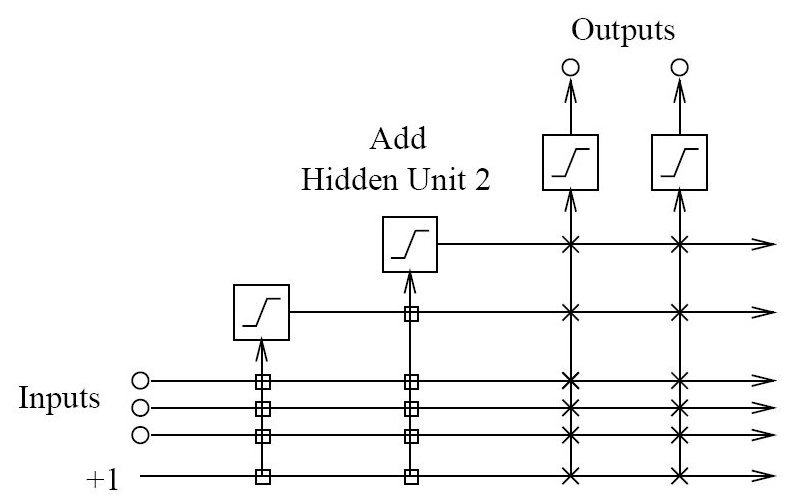
\includegraphics[scale=0.50]{cascade_net}
		\caption[The Cascade-Correlation architecture]{The Cascade-Correlation architecture after adding two hidden units. Each new hidden unit receives a connection from both every original input units and pre-existing hidden units. Its input weights are frozen at the time the unit is added to the net. This fact is represented with boxed connections ($\Box$). Instead, output connections, described as cross connections ($\times$) are trained repeatedly.}
		\label{fig:cascade_net}
	\end{center}
\end{figure}


\subsubsection{Validation}
\label{subsubsec:validation}
The choice for the best parameters to configure a neural network is a fundamental and difficult aspect that determines the quality of the predictor. Only the most important parameters are investigated in order to fit the best values. For fixed topology ANNs, the number of epochs and hidden units are taken into account, in the range $[1, 5000]$ with step $250$ and $[2, 5]$ with step $1$ respectively.
For variable topology ANNs, only the number of hidden units is considered in the range $[1, 25]$ with step $1$.\\
With the intent of having a better accuracy for the generated ANN, K-fold cross validation is used. This technique consists in creating a K-fold partition of the dataset (TR + VA). For each of the K experiments, $K-1$ folds are used for training and the remaining one for validating the obtained ANN, as shown in Figure \ref{fig:kfoldcrossvalidation}. The advantage of K-fold cross validation over other techniques, e.g. Random Subsampling, is that all dataset samples are eventually used for both training and testing. The true error is estimated as the average error rate:
 \begin{equation}
  	\tilde{E} = \frac{1}{K}\sum_{i=1}^{K}E_i
 \end{equation}
where $E_i$ is the MSE when the validation set is the $i$-th fold. 

\begin{figure}[tb]
	\begin{center}
		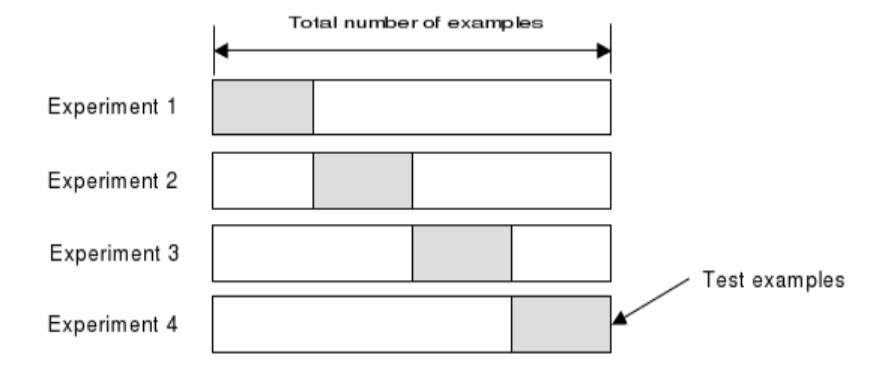
\includegraphics[scale=0.65]{kfoldcrossvalidation}
		\caption[K-fold cross validation]{Example of K-fold cross validation.}
		\label{fig:kfoldcrossvalidation}
	\end{center}
\end{figure}
In order to achieve small values for the \glslink{bias}{bias} and \glslink{variance}{variance} of the true error rate estimator and to reduce computation time, the parameter K is set to $5$. In fact, with a large number of folds, the bias will be small (that means that the estimator will be very accurate), but the variance and computation time (that depend on the number of experiments) will be very large. On the other hand, with a small number of folds, the variance and computation time are reduced, but the bias of the estimator will be large. Moreover, since the original training set, composed by both TR and VA is very large, $5$-fold cross validation yields a good accuracy. A review about the most important accuracy estimation methods can be found in \cite{Kohavi1995}.
% folds obtained by using (mod 4). no data randomization before splitting into folds. skip

\subsubsection{Testing}
\label{subsubsec:testing}
The implemented individual methods are very fast. In fact, after having trained the neural network, the execution involves only the information processing from input to output units. Although the training process requires several hours to complete, due to the training set width, the running process only depends on the number of neural units that are used and this number is constant. In order to test the network performance, two different datasets are used, one from CASP-4 and the other from CASP-8. The first is made of relatively simple targets, while the second, proposed in 2008, comprises a wide target set of different difficulty for quality assessment. Performance evaluation is usually based on a measure of global correlation. This measure also allows to compare the implemented method with other related work. Here, correlation indicates a linear relationship between two random variables that represent the true and predicted score, giving a value in the range $[-1,+1]$. If the correlation is $1$, then the two random variables are identical. The correlation reflects only the noisiness and direction, but not the slope of that relationship.
At CASP, the measure to assess a model score is GDT\_TS. The true score of a model can be obtained by using the program TMscore measuring the similarity between the given protein model and the relative native structure. The predicted score of a model is determined by the MQAP. Here, the focus is on the global correlation of a method, which stands for the correlation whose data are all models of all given targets. The Pearson and Spearman correlations are used together in order to understand more accurately the results. Moreover, for the CASP-8 test set, a comparison with the best MQAPs is provided.



\subsection{Target Categorization}
\label{subsec:target_categorization}
The idea is to handle targets differently with respect to their category in order to increase the accuracy in general. Hence, a formulation of categorization and a manner to use the classification information are required. The key point is that models are generated by different types of tertiary structure predictors and this information determines the obtained model quality. Figure \ref{fig:model_distribution_in_casp567} reports the quality distribution of models coming from CASP-5, CASP-6 and CASP-7.
\begin{figure}[tb]
	\begin{center}
		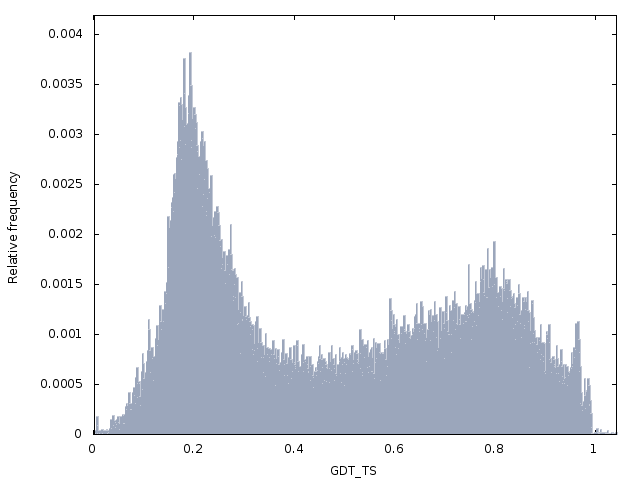
\includegraphics[scale=0.60]{model_distribution_in_casp567}
		\caption[Mixture of Gaussian distributions describing the model frequency with respect to the quality]{Mixture of Gaussian distributions describing the model frequency with respect to the quality. Distributions are obtained by using 78,854 models from CASP-5, CASP-6 and CASP-7.}		
		\label{fig:model_distribution_in_casp567}
	\end{center}
\end{figure}
Two main Gaussian distribution are separated approximately at the threshold $\theta = 0.41$ GDT\_TS. The first distribution contains raw or wrong models typically obtained by using \emph{ab initio} or \emph{novel fold} methods. These models are called \glslink{FM}{Free Models (FM)}. The second one instead contains more accurate models mostly obtained by using comparative modelling or fold recognition techniques. These models are called \glslink{TBM}{Template-Based Models (TBM)}. A more detailed distinction could further be achieved in the TBM distribution. In fact, it could be split again into medium and high quality classes, as shown in Figure approximately at the threshold $\psi = 0.77$ GDT\_TS. By this distinction, models with score in the range $(\theta,\psi]$ are called TBM, whereas models with score greater than $\psi$ are called \glslink{HQM}{High Quality Models (HQM)}. This last distribution contains models that are very similar to the native structure. Therefore, an accurate quality assessment for HQM models is much more important than that for TBM or FM models. The goal is to apply this classification also to the implemented method, in order to refine the prediction method (see Figure \ref{fig:system_execution}), while considering target instead of model classification. The idea is to decompose a problem so that it is dealt with by three modular expert components (FM\_ANN, TBM\_ANN and HQM\_ANN), each of which is designed as a specific function approximator \cite{Sharkey96aa,MuiAGW94aa,FrosyniotisSL03aa,Happel1994aa,Schmidt1996aa}. In this way, every component of the neural network system can be different from the others by varying the architecture, feature space (see \S~\ref{subsec:addition_of_new_features}) and dataset. By adopting a modular architecture, each module could be trained in parallel, improving the computation time. Also, by splitting the dataset into classes and training a module using only data from a class, the non-linear function to learn is obviously simpler, because more specific, and thus the training is faster. 
Algorithm \ref{algo:target_classification} describes the target classification.
\begin{algorithm}
\caption{$ClassifyTarget(Target)$}
\label{algo:target_classification}
\begin{algorithmic}[1]
\REQUIRE $Target \neq \emptyset$
\ENSURE $Target$ is classified
\STATE $\theta \leftarrow 0.41$
\STATE $\psi \leftarrow 0.77$
\STATE $\tilde{t} \leftarrow MedianScore(Target))$
\STATE $Class(Target) \leftarrow null$
\IF{$\tilde{t} \leq \theta$}
	\STATE $Class(Target) \leftarrow FM$
\ELSIF{$\tilde{t} \leq \psi$}
	\STATE $Class(Target) \leftarrow TBM$
\ELSE [$\tilde{t} > \psi$]
	\STATE $Class(Target) \leftarrow HQM$
\ENDIF
\RETURN $Class(Target)$
\end{algorithmic}
\end{algorithm}
The median is preferred in this case over the mean because it is more robust regarding outliers. An outlier is an observation that is numerically distant from the rest of the data, generating skewed distributions. For each target sequence, models typically form a skewed distribution since FM predictors build many more models than TBM or HQM predictors. The median better balances this fact.\\
Target classification is proposed instead of model classification as it allows to associate a class by considering a set of models. Methods learn better by using target classification since classes are not completely disjoint, but contain overlapping information that is characterized by models (outliers) that would belong to a different class with respect to their target one.
\begin{figure}[tb]
	\begin{center}
		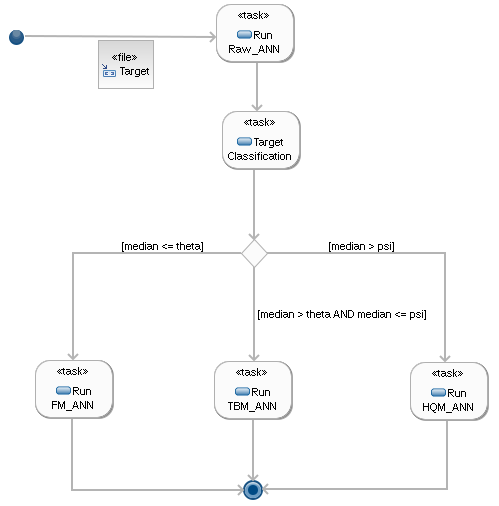
\includegraphics[scale=0.85]{system_execution}
		\caption[Control flow of the neural system]{UML activity diagram showing the control flow of the neural system. A raw ANN is trained without considering differences in the distribution of models. Three expert ANNs are trained only on specific classes: FM, TBM and HQM. ANNs compute a GDT\_TS score in the range $[0, 1]$. For each target, the median of model scores that have been predicted by the Raw\_ANN is calculated. In this way, the Raw\_ANN is used both to predict a score for each model and to classify targets. After being categorized, a target is sent to the expert ANN associated to its class. There is no score combination at the end of the process, as common in modular approaches, but only a data splitting after applying the Raw\_ANN.}
		\label{fig:system_execution}
	\end{center}
\end{figure}


\subsection{Density Information}
\label{subsec:density_information}
Clustering methods are recognized to be very accurate in model quality assessment. In this kind of programs, a set of models is evaluated by considering similarities among models. The idea is to use the density information after having applied a MQAP method, e.g. QMEAN or ANN with features from QMEAN. In order to measure similarities between two models, the GDT\_TS quality measure is adopted. Given two models $m$ and $n$, the GDT\_TS similarity has, by definition, the following properties:
\begin{enumerate}
 \item $GDT\_TS(m, n) \geq 0$ and $GDT\_TS(m, n) \leq 1$.
 \item $GDT\_TS(m, n) = 1$ if and only if $m = n$.
 \item $GDT\_TS(m, n) = GDT\_TS(n, m)$.
\end{enumerate}
It is important to highlight that the GDT\_TS measure is not a distance since it does not satisfy the triangle inequality. This fact is shown by using a counterexample. Given three models $r$, $s$ and $t$ where $r$ and $s$ are very similar, e.g. $x = GDT\_TS(r, s) = 0.9$, while $t$ is very different from the previous two models, e.g. $y = GDT\_TS(r, t) = 0.1$ and $z = GDT\_TS(s, t) = 0.2$, in order to satisfy the triangle inequality, the following conditions must be valid $x \leq y + z$, $y \leq x + z$ and $z \leq x + y$. However the first condition is false because $0.9 \nleq 0.1 + 0.2$.\\
A similarity matrix is computed for any target $T$ by computing the GDT\_TS between each pair of target models. This matrix is squared, symmetric and has diagonal $1$ due to the above properties. Thus, only the upper or lower triangle with respect to the diagonal needs to be computed. In other words the matrix describes the similarities of each model with respect to the others. Therefore, the clustering process serves to calculate a score that takes into account the similarities between the current model and the other models. \\
Instead of considering all models to assess the score of a given model, a better solution is to use only a subset of the best models, building up a semi-clustering procedure. The idea is to limit the well-known clustering drawback, that is the loss of the best models which are far from the center of the main cluster. Very bad models represent outliers in the whole target distribution and, for this reason, should be eliminated from the clustering computation. The semi-clustering approach is illustrated in Figure \ref{fig:semi_clustering}.\\
\begin{figure}[tb]
	\begin{center}
		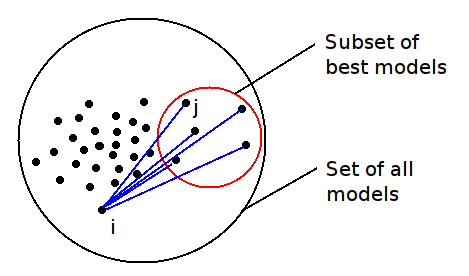
\includegraphics[scale=0.8]{semi_clustering}
		\caption[The semi-clustering approach]{The semi-clustering approach. A previous MQAP (e.g QMEAN) provides an estimation of the quality of each target model. An optimized percentage value, computed over target models of CASP-5, CASP-6 and CASP-7 and specific for FM, TBM and HQM targets, defines the size of the best subset. In this semi-clustering approach, only the subset of the best models is dealt with, instead of considering all target models. The lines between model $i$ and models in the best subset represent the similarities (not the distances). In order to score model $i$, the mean of these similarities, weighted by the previous MQAP scores of the best models used, is calculated. Finally, the computed mean is weighted by the $PFractionModelled$ of the model $i$.}
		\label{fig:semi_clustering}
	\end{center}
\end{figure}
A way to obtain such a subset is to consider a percentage of the best scores achieved by an other MQAP, i.e. QMEAN, used as support method. A specific percentage is optimized over target models from CASP-5, CASP-6 and CASP-7 datasets for the FM, TBM and HQM targets, using QMEAN as support MQAP (see \S~\ref{subsec:semiclustering_optimization}). The best percentages are obtained in the following way. First of all, targets are split into the three categories FM, TBM and HQM. Therefore, for each class, by varying the percentage of the best models, each target is clustered and a class Pearson correlation is computed between the cluster scores and the real scores. Finally, the best percentage of each class, that is the value corrisponding to the highest Pearson correlation for the class, is found. The optimization plots for FM, TBM and HQM models respectively are proposed in \S~\ref{subsec:semiclustering_optimization}. Algorithm \ref{algo:optimize_percentages} describes the optimization.\\
% NOTE: NO \COMMENT{} directly after \FOR |WHILE |FORALL loops
\begin{algorithm}
\caption{$OptimizePercentages(Targets)$}
\label{algo:optimize_percentages}
\begin{algorithmic}[1]
\REQUIRE $Targets \neq \emptyset$
\ENSURE A percentage for each class (FM, TBM, HQM)
\STATE $FMset \leftarrow \{T \in Targets$ such that $Class(T) = FM\}$
\STATE $TBMset \leftarrow \{T \in Targets$ such that $Class(T) = TBM\}$
\STATE $HQMset \leftarrow \{T \in Targets$ such that $Class(T) = HQM\}$
\STATE $Classes \leftarrow \{FMset, TBMset, HQMset\}$
\FOR{each class $C$ such that $C \in Classes$}
	\STATE $RealScores \leftarrow \emptyset$
	\FOR{each target $T$ such that $T \in C$}
		\STATE $Add(RealScores, RealScore(T))$
	\ENDFOR	
	\FOR{$\lambda=0.05$ step $0.01$ to $1.0$}
		\STATE $PERCENTAGE_C \leftarrow \lambda$
		\STATE $ClusterScores \leftarrow \emptyset$
		\FOR{each target $T$ such that $T \in C$}
			\STATE $Add(ClusterScores, Clustering(T))$
		\ENDFOR
		\STATE $Pearson \leftarrow PearsonCorrelation(RealScores, ClusterScores))$
		\PRINT $(\lambda, Pearson)$
	\ENDFOR
\ENDFOR
\end{algorithmic}
\end{algorithm}
Sometimes a predicted model is incomplete, in the sense that only a part of the target sequence is modelled. The $FractionModelled$ feature, computed by QMEAN, represents the percentage of modelled structure. By applying the $FractionModelled$ descriptor, the effect gained is to reduce the final scores of incomplete models. In other terms, it lowers the presence of false positive models, e.g. structures where the modelled part is well predicted, causing the MQAP to assign a high score to those models, regardless of being incomplete. By weighting models for their fraction modelled, more correct scores are achieved. However, the pure $FractionModelled$ application sometimes penalizes too much the model scores. In order to overcome this drawback, a solution may be to use another feature computed from the known $FractionModelled$. The aim is that this new feature does not penalize too much nearly complete models but is able to lower the score of false positive models previously discussed. A function that satisfies these requirements is the following:
 \begin{equation}
  	f(x) = -x^2 + 2x
 \end{equation}
where $x \in [0, 1]$ is the common $FractionModelled$ feature. This new function, called $PFractionModelled$, where $P$ stands for Parabolic, performs better than the usual one as shown in \S~\ref{subsec:parabolic_fraction_modelled}. Figure \ref{fig:parabolic_fraction_modelled} shows the function $PFractionModelled$. 
\begin{figure}[tb]
	\begin{center}
		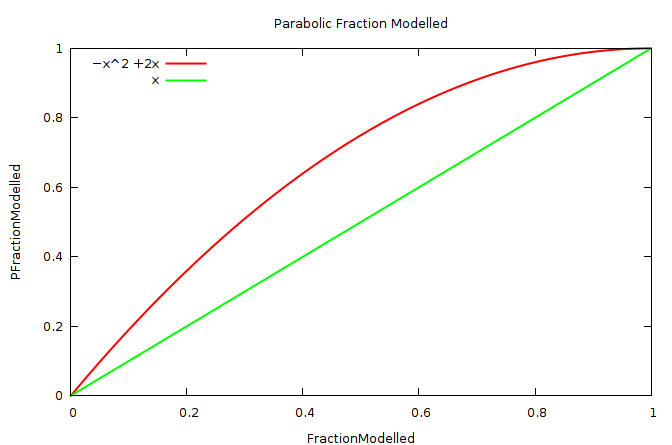
\includegraphics[scale=0.6]{parabolic_fraction_modelled}
		\caption[Parabolic Fraction Modelled function]{Parabolic Fraction Modelled function. By using this function, cluster scores are less affected by the computed fraction modelled of the structure.}
		\label{fig:parabolic_fraction_modelled}
	\end{center}
\end{figure}
It is important to highlight that the $FractionModelled$ feature is purely quantitative because it does not take into account that protein regions may have different importance. For example, given two identical protein models, their $FractionModelled$ could be the same also if the first one misses a piece of polypeptide backbone concerning the active site whereas the second a piece less important. However, the second model quality is clearly greater than the first one. Computing a $FractionModelled$ in order to consider differently the modelled parts is a hard task because it needs to recognize which parts are more important than others. The $PFractionModelled$ feature implicitly assumes that small faults in the model constitute almost trascurable errors, whereas larger faults represent important mistakes. This assumption is consistent with the observed data (see \S~\ref{sec:protein_structure_prediction}).\\
Algorithms \ref{algo:get_discrimination_score} and \ref{algo:target_clustering} describe the clustering subroutines.
\begin{algorithm}
\caption{$DiscriminatingScore(Target)$}
\label{algo:get_discrimination_score} 
\begin{algorithmic}[1]
\REQUIRE $Target \neq \emptyset$
\ENSURE The score of the worst model $m \in BestModels(Target)$. This score discriminates the best models from all others.
\STATE $\tau \leftarrow PERCENTAGE_{Class(Target)}$
\COMMENT{$PERCENTAGE_{Class(Target)} \in (0,1]$ is the optimized percentage referred to the $Target$ class. Classes are FM, TBM and HQM.}
\STATE $SortedScore \leftarrow Score(Target)$
\STATE $n \leftarrow Size(SortedScore)$
\FOR{each model $m$ such that $m \in Target$}
	\STATE $SortedScore[m] \leftarrow SortedScore[m] * PFractionModelled(Target, m)$
\ENDFOR
\STATE $SortedScore \leftarrow Sort(SortedScore)$
\STATE $DiscrimPos \leftarrow n - (n * \tau)$
\COMMENT{If $\tau \rightarrow 0^{+}$ then $DiscrimPos \rightarrow n^{-}$. Due to approximations this could lead to a buffer overflow of one element. By assumption, the element in position $(DiscrimPos-1)$ always exists and corresponds to the last (the greatest) element of $SortedScores$.}
\IF{$DiscrimPos = n$}
	\RETURN $SortedScore[DiscrimPos - 1]$
\ENDIF
\RETURN $SortedScore[DiscrimPos]$
\end{algorithmic}
\end{algorithm}
\begin{algorithm}
\caption{$Clustering(Target)$}
\label{algo:target_clustering}
\begin{algorithmic}[1]
\REQUIRE $Target \neq \emptyset$
\ENSURE A new score for each model $m \in Target$
\STATE $Sum \leftarrow 0$
\STATE $WeightedSum \leftarrow 0$
\STATE $TempScore \leftarrow 0$
\STATE $Threshold \leftarrow DiscriminatingScore(Target)$
\STATE $ClusterScore(Target) \leftarrow \emptyset$
\FOR{each model $m$ such that $m \in Target$}
	\STATE $Sum \leftarrow 0$
	\STATE $WeightedSum \leftarrow 0$
	\FOR{each model $n$ such that $n \in Target$}
		\IF{$Similarity(Target, m, n) \neq 0$ and\\ 
		    $(Score(Target, n) * PFractionModelled(Target, n)) \geq Threshold$}
			\STATE $Sum \leftarrow Sum + Score(Target, n)$
			\STATE $WeightedSum \leftarrow WeightedSum + $\\
			       $(Similarity(Target, m, n) * Score(Target, n))$
			\COMMENT{$Score(Target, n)$ is not weighted by $PFractionModelled(Target, n)$.}
		\ENDIF
	\ENDFOR
	\STATE $TempScore \leftarrow (WeightedSum / Sum) * PFractionModelled(Target, m)$
	\STATE $Add(ClusterScores(Target), TempScore)$
\ENDFOR
\RETURN $ClusterScores(Target)$
\end{algorithmic}
\end{algorithm}
The algorithm used to cluster target models has a running time of $0(n^{2})$ where $n$ is the number of models proposed for a certain target. In practice, $n$ has values between $200$ and $400$. To improve the method performance, the similarity matrices can be computed once previously to the clustering process.



\subsection{Addition of New Features}
\label{subsec:addition_of_new_features}
The last approach adopted to improve QMEAN includes the addition of new features. Feature selection is an important, but also hard, task that has the aim to find a set of effective, non redundant and independent protein descriptors. The intent is to define new ANNs based on features retrieved from both QMEAN and other methods.\\
Three new features are taken into account: Gauss integrals, hydrogen bonds and TAP score. The following subsections describe these features and how they are combined together with QMEAN. All additional features, with ranges in the interval $[0, 1]$, are scaled by using the equation \ref{eq:feature_normalization}.

\subsubsection{Gauss Integrals}
\label{subsubsec:gauss_integrals}
An interesting and new way to describe proteins from a geometrical point of view is represented by Gauss integrals \cite{Rogen2005,Rogen2003,Rogen2003b}. They are protein shape descriptors, independent of translation and rotation, that are able to distinguish among similar, but still different morphologies. Generalized Gauss integrals arise from Vasiliev knot invariants and deal with crossings seen in all planar projections of curves representing the protein polypeptide chain. Crossings have a sign defined by the right-hand rule (see Figure \ref{fig:link_crossings}). The generalized Gauss integrals used in this work are based on the writhe and average crossing number of first, second and third orders. The writhe is the total number of positive crossings minus the total number of negative crossings, whilst the average crossing number of a curve is the unsigned average number of crossings seen in the different planar projections of the curve (see Figure \ref{fig:labeled_whitehead_link}).
\begin{figure}[tb]
	\begin{center}
		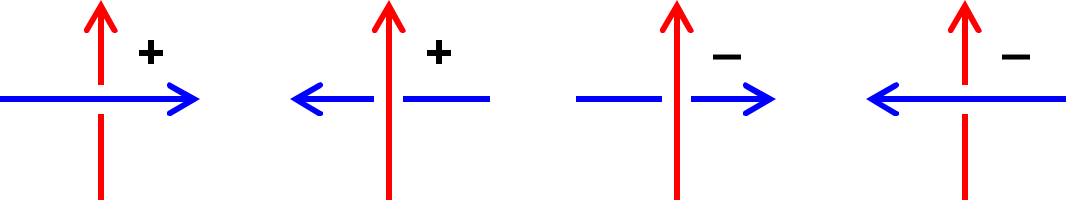
\includegraphics[scale=0.35]{link_crossings}
		\caption[Positive and negative crossings]{Examples of positive and negative crossings.}
		\label{fig:link_crossings}
	\end{center}
\end{figure}
\begin{figure}[tb]
	\begin{center}
		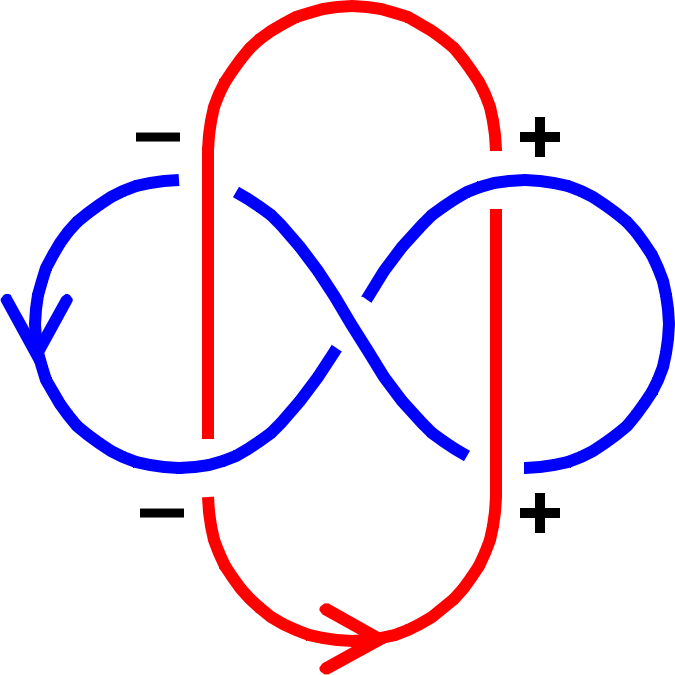
\includegraphics[scale=0.30]{labeled_whitehead_link}
		\caption[Example of crossings seen in two curves]{Example of crossings seen in two curves.}
		\label{fig:labeled_whitehead_link}
	\end{center}
\end{figure}
A more detailed explanation and formalization of Gauss integrals is reported in Appendix \ref{appendix:gauss_integrals}.
The program used to compute Gauss integrals is called \gls{GIT}. GIT can operate in two modes. The first calculates Gauss integrals by considering exactly protein backbone $C_\alpha$ atoms, whereas the second deals with a \emph{smoothed} version of the protein backbone. The first mode is chosen by exclusion, because the second one is not stable in the generation of Gauss integrals. The low reliability of the results for the second mode might be associated to the fact that protein models and not experimental structures are considered in this work. 
Instead of using all computed $29$ descriptors, the most informative ones, i.e. the more discriminative among all $29$ Gauss integrals, are taken into account by considering Ba\'{u}'s work \cite{Bau2008}. The following $7$ Gauss invariants were selected: $I_{(1,2)}$, $I_{(1,2)(3,4)}$, $I_{(1,2)(3,4)(5,6)}$, $I_{(1,2)(3,5)(4,6)}$, $I_{(1,2)(3,6)(4,5)}$, $I_{(1,4)(2,3)(5,6)}$ and $I_{(1,6)(2,3)(4,5)}$. 



\subsubsection{Hydrogen Bonds}
\label{subsubsec:hydrogen_bonds}
A hydrogen bond is the attractive force between an electronegative atom and a hydrogen covalently bound to another electronegative atom. It results from a dipole-dipole force with a hydrogen atom bound to fluorine, nitrogen or oxygen (see Figure \ref{fig:os_wat2}).
These bonds can occur between molecules (intermolecularly), or within different parts of a single molecule (intramolecularly). A hydrogen bond is a very strong fixed dipole-dipole van der Waals force, but weaker than covalent, ionic bonds. It is somewhere between a covalent bond and an electrostatic intermolecular attraction. This type of bond occurs in both inorganic molecules (such as water) and organic molecules (such as DNA) (see Figure \ref{fig:quadruple_hydrogen_bond}). 
The length of hydrogen bonds depends on bond strength, temperature, and pressure. The bond strength itself is dependent on temperature, pressure, bond angle, and environment. The typical length of a hydrogen bond in water is 1.97 \AA.\\
Hydrogen bonds plays an important role in determining the three-\-di\-men\-sio\-nal protein structures. In such macromolecules, bonds between parts of the same macromolecule are partially responsible to the folding process. Hydrogen bonds form between the backbone oxygens and amide hydrogens and contribute to the formation of alpha helices and beta sheets. Hydrogen bonds also play a part in forming the tertiary structure of proteins through interaction of $R$-groups. For these reasons, the use of hydrogen bond-based features should be relevant. In order to compute hydrogen bonds, the program HBPLUS \cite{McDonald1994aa} is adopted. The application returns the number of hydrogen bonds found in a three-\-di\-men\-sio\-nal protein and this number is used as feature.
\begin{figure}[tb]
	\begin{center}
		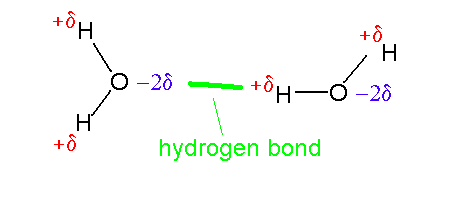
\includegraphics[scale=0.70]{os_wat2}
		\caption[Example of hydrogen bond between two water molecules]{Example of hydrogen bond between two water molecules.}
		\label{fig:os_wat2}
	\end{center}
\end{figure}

\begin{figure}[tb]
	\begin{center}
		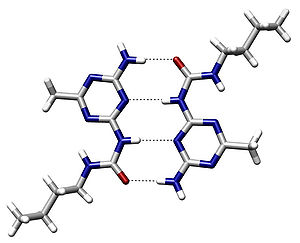
\includegraphics[scale=0.80]{quadruple_hydrogen_bond}
		\caption[Example of intermolecular hydrogen bonding]{Example of intermolecular hydrogen bonding in a self-assembled dimer complex (See \cite{Beijer1998sca}).}
		\label{fig:quadruple_hydrogen_bond}
	\end{center}
\end{figure}

\subsubsection{TAP score}
\label{subsubsec:tap_score}
TAP score \cite{Tosatto2007aa} is a recent criterion for measuring, in a quantitative way, the sequence to structure compatibility based on the normalization of torsion angle propensities including the side chain. The normalization involves the definition of the global minimum and maximum of the protein sequence. TAP score is used to recognize the best experimental structures.\\
TAP score estimates the quality of a protein model based on the Ramachandran plot of the backbone ($\phi$, $\psi$) torsion angles, thus it is based on conformational criteria. While each amino acid type may, in theory, adopt a large number of different conformations, here, large areas of the Ramachandran plot are almost empty. This is due to steric clashes deriving from the local geometry of the polypeptide chain. TAP score simultaneously combines five different torsion angles into a single pseudo-energy value. Adding more torsion angles is known to improve the overall discrimination of protein decoys, as it captures the subtle interplay between them. TAP score explores the avenue of capturing the interplay between protein backbone and side chain. \\
One benefit of adopting a modular approach to ANNs is the possibility to employ a set of specific features for a certain module of the neural system \cite{Happel1994aa}. Since TAP score is indicative to assess scores for high quality structures, the idea is to use it as a feature for only high quality targets that are predicted by the HQM expert ANNs.

%    - the final system (QMEAN + raw_ann + expert_anns + cluster)


\cleardoublepage
